
%\documentclass[mathserif]{beamer}
\documentclass[handout]{beamer}
%\usetheme{Goettingen}
%\usetheme{Warsaw}
\usetheme{Singapore}



%\usetheme{Frankfurt}
%\usetheme{Copenhagen}
%\usetheme{Szeged}
%\usetheme{Montpellier}
%\usetheme{CambridgeUS}
%\usecolortheme{}
%\setbeamercovered{transparent}
\usepackage[english, activeacute]{babel}
\usepackage[utf8]{inputenc}
\usepackage{amsmath, amssymb}
\usepackage{dsfont}
\usepackage{graphics}
\usepackage{cases}
\usepackage{graphicx}
\usepackage{pgf}
\usepackage{epsfig}
\usepackage{amssymb}
\usepackage{multirow}	
\usepackage{amstext}
\usepackage[ruled,vlined,lined]{algorithm2e}
\usepackage{amsmath}
\usepackage{epic}
\usepackage{epsfig}
\usepackage{fontenc}
\usepackage{framed,color}
\usepackage{palatino, url, multicol}
%\algsetup{indent=2em}
\newcommand{\factorial}{\ensuremath{\mbox{\sc Factorial}}}
\newcommand{\BIGOP}[1]{\mathop{\mathchoice%
{\raise-0.22em\hbox{\huge $#1$}}%
{\raise-0.05em\hbox{\Large $#1$}}{\hbox{\large $#1$}}{#1}}}
\newcommand{\bigtimes}{\BIGOP{\times}}
\vspace{-0.5cm}
\title{Natural Language Processing \\ Text Classification and Naïve Bayes}
\vspace{-0.5cm}
\author[Felipe Bravo Márquez]{\footnotesize
%\author{\footnotesize  
 \textcolor[rgb]{0.00,0.00,1.00}{Felipe Bravo-Marquez}} 
  
 

\date{\today}

\begin{document}
\begin{frame}
\titlepage


\end{frame}



\begin{frame}{Is this spam?}

\begin{figure}[h]

\includegraphics[scale = 0.35]{pics/spam.png}
\end{figure}


\begin{scriptsize}
This slides are based on the course material by Daniel Jurafsky : \url{https://web.stanford.edu/~jurafsky/slp3/4.pdf} 
\end{scriptsize}
\end{frame}

\begin{frame}{Who wrote which Federalist papers?}
    \scriptsize
    \begin{itemize}
        \item 1787-8: Anonymous essays attempted to convince New York to ratify the U.S Constitution: Jay, Madison, Hamilton.
        \item Authorship of 12 of the letters is in dispute.
        \item 1963: Solved by Mosteller and Wallace using Bayesian methods.
    \end{itemize}
    \vspace{5pt}
    \begin{center}
        \begin{figure}[h]
            \begin{minipage}{0.3\textwidth}
                \centering
                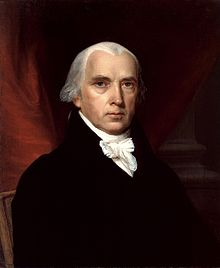
\includegraphics[width=\linewidth]{pics/madison.png}
                \caption{James Madison}
            \end{minipage}\hfill
            \begin{minipage}{0.3\textwidth}
                \centering
                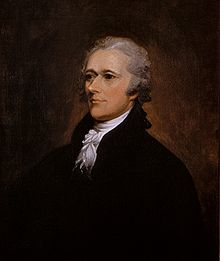
\includegraphics[width=\linewidth]{pics/hamilton.png}
                \caption{Alexander Hamilton}
            \end{minipage}
        \end{figure}
    \end{center}
\end{frame}

\begin{frame}{What is the subject of this medical article?}

\begin{figure}[h]
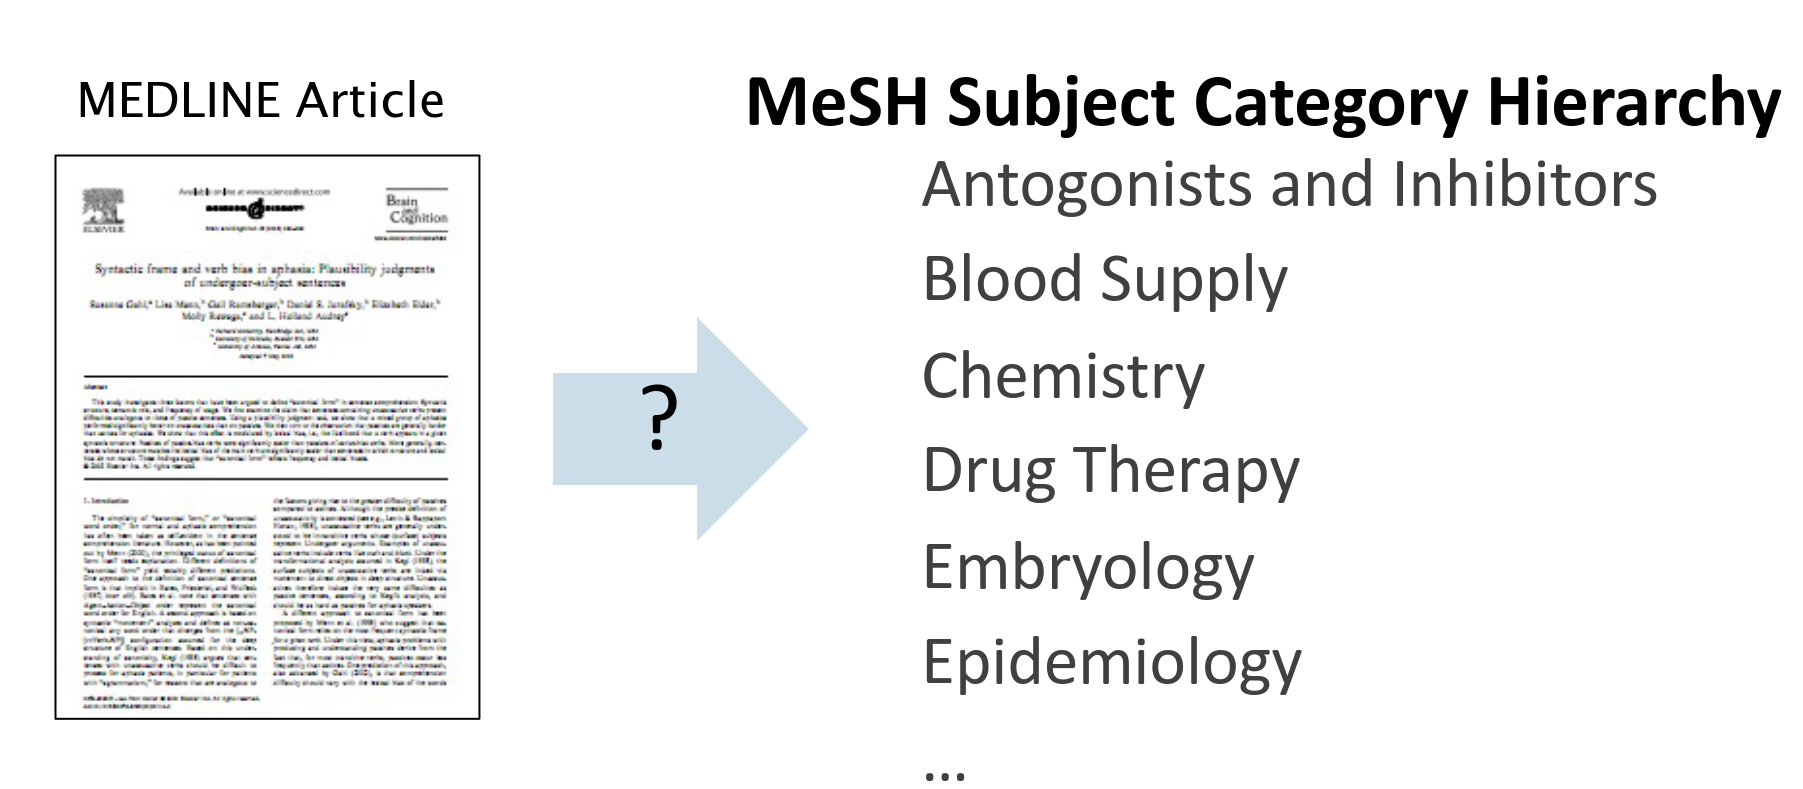
\includegraphics[scale = 0.2]{pics/medarticle.png}
\end{figure}


\end{frame}


\begin{frame}{Positive or negative movie review?}
    \begin{itemize}
     \item  \textcolor{blue}{\textbf{+}}   ...zany characters and \textcolor{blue}{richly} applied satire, and some \textcolor{blue}{great} plot twists 
     \item   \textcolor{red}{\textbf{-}} It was \textcolor{red}{pathetic}. The \textcolor{red}{worst} part about it was the boxing scenes... 
    \item   \textcolor{blue}{\textbf{+}}  ...\textcolor{blue}{awesome} caramel sauce and sweet toasty almonds. I \textcolor{blue}{love} this place! \\
     \item \textcolor{red}{\textbf{-}} ...\textcolor{red}{awful} pizza and \textcolor{red}{ridiculously} overpriced... 
    \end{itemize}

\end{frame}

\begin{frame}{Why sentiment analysis?}
    \begin{itemize}
        \item Movie: Is this review positive or negative?
        \item Products: What do people think about the new iPhone?
        \item Public sentiment: How is consumer confidence?
        \item Politics: What do people think about this candidate or issue?
        \item Prediction: Predict election outcomes or market trends from sentiment.
    \end{itemize}
\end{frame}

\begin{frame}{Scherer Typology of Affective States}
    \scriptsize
    \begin{itemize}\scriptsize
        \item Emotion: Brief organically synchronized ... evaluation of a major event
        \begin{itemize}\scriptsize
            \item Angry, sad, joyful, fearful, ashamed, proud, elated
        \end{itemize}
        \item Mood: Diffuse non-caused low-intensity long-duration change in subjective feeling
        \begin{itemize}\scriptsize
            \item Cheerful, gloomy, irritable, listless, depressed, buoyant
        \end{itemize}
        \item Interpersonal stances: Affective stance toward another person in a specific interaction
        \begin{itemize}\scriptsize
            \item Friendly, flirtatious, distant, cold, warm, supportive, contemptuous
        \end{itemize}
        \item Attitudes: Enduring, affectively colored beliefs, dispositions towards objects or persons
        \begin{itemize}\scriptsize
            \item Liking, loving, hating, valuing, desiring
        \end{itemize}
        \item Personality traits: Stable personality dispositions and typical behavior tendencies
        \begin{itemize}\scriptsize
            \item Nervous, anxious, reckless, morose, hostile, jealous
        \end{itemize}
    \end{itemize}
\end{frame}

\begin{frame}{Basic Sentiment Classification}
    Sentiment analysis is the detection of attitudes.
    \begin{itemize}
        \item Simple task we focus on in this class
        \begin{itemize}
            \item Is the attitude of this text positive or negative?
        \end{itemize}
    \end{itemize}
\end{frame}


\begin{frame}{Summary: Text Classification}
    Text classification can be applied to various tasks, including:
    \begin{itemize}
        \item Sentiment analysis
        \item Spam detection
        \item Authorship identification
        \item Language identification
        \item Assigning subject categories, topics, or genres
        \item ...
    \end{itemize}
\end{frame}

\begin{frame}{Text Classification: Definition}
    \textbf{Input}:
    \begin{itemize}
        \item A document $d$
        \item A fixed set of classes $C = \{c_1, c_2, \ldots, c_J\}$
    \end{itemize}
    
    \textbf{Output}: A predicted class $c \in C$
\end{frame}

\begin{frame}{Classification Methods: Hand-coded rules}
    Rules based on combinations of words or other features
    \begin{itemize}
        \item Spam: \textit{black-list-address} OR (\textit{“dollars” AND “you have been selected”})
        \item Accuracy can be high if rules carefully refined by experts
        \item But building and maintaining these rules is expensive
    \end{itemize}
\end{frame}

\begin{frame}{Classification Methods: Supervised Machine Learning}
    \textbf{Input}:
    \begin{itemize}
        \item A document $d$
        \item A fixed set of classes $C = \{c_1, c_2, \ldots, c_J\}$
        \item A training set of $m$ hand-labeled documents: $(d_1, c_1), (d_2, c_2), \ldots, (d_m, c_m)$
    \end{itemize}
    
    \textbf{Output}:
    \begin{itemize}
        \item A learned classifier $\gamma: d \to c$
    \end{itemize}
\end{frame}

\begin{frame}{Classification Methods: Supervised Machine Learning}
    Any kind of classifier can be used:
    \begin{itemize}
        \item Naïve Bayes
        \item Logistic regression
        \item Neural networks
        \item k-Nearest Neighbors
        % Add more classifiers as needed
    \end{itemize}
\end{frame}

\begin{frame}{Naive Bayes Intuition}
    Naive Bayes is a simple ("naive") classification method based on Bayes' rule.
    \begin{itemize}
        \item Relies on a very simple representation of a document: \textit{Bag of words}
    \end{itemize}
\end{frame}

\begin{frame}{The Bag of Words Representation}

\begin{figure}[h]
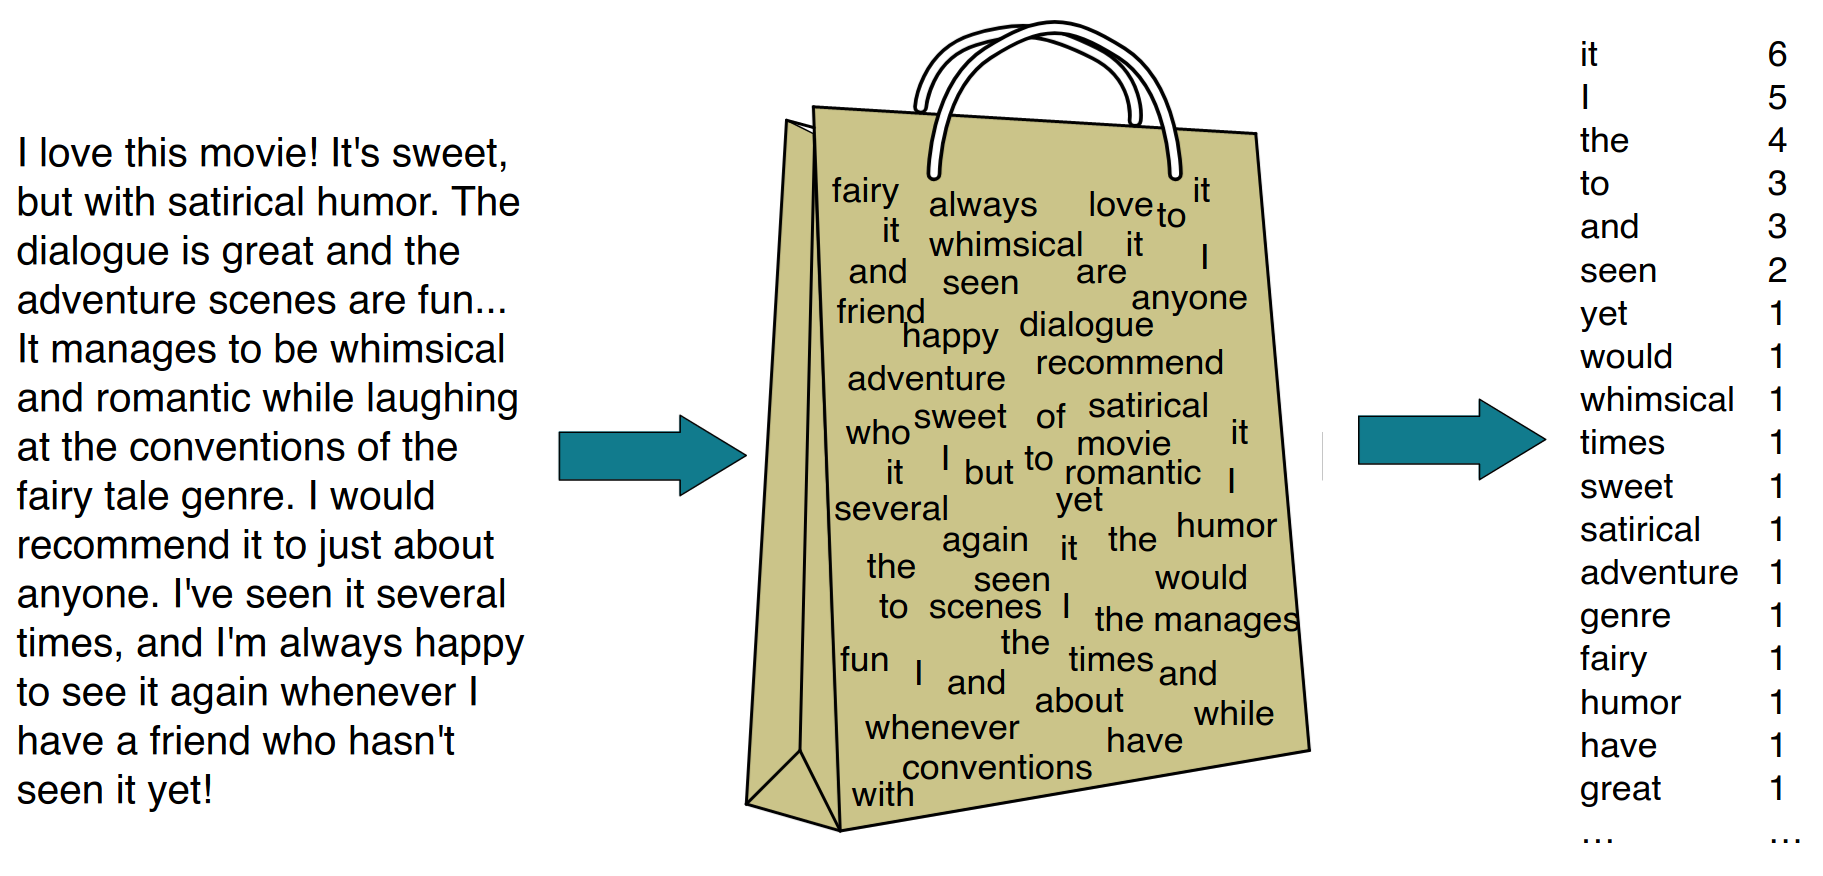
\includegraphics[scale = 0.22]{pics/bow.png}
\end{figure}


\end{frame}

\begin{frame}{Bayes' Rule Applied to Documents and Classes}
    For a document $d$ and a class $c$:
    \[
    P(c | d) = \frac{P(d | c)P(c)}{P(d)}
    \]
\end{frame}

\begin{frame}{Naive Bayes Classifier (I)}
\scriptsize
\begin{itemize}
    \item MAP stands for "maximum a posteriori," which represents the most likely class:
    \[
    c_{\text{MAP}} = \arg\max_{c \in C} P(c | d)
    \]
    \item To calculate the most likely class, we apply Bayes' rule:
    \[
    = \arg\max_{c \in C} \frac{P(d | c)P(c)}{P(d)}
    \]
    \item Finally, we can drop the denominator since it remains constant for all classes:
    \[
    = \arg\max_{c \in C} P(d | c)P(c)
    \]
\end{itemize}
\end{frame}

\begin{frame}{Naive Bayes Classifier (II)}
\scriptsize
\begin{itemize}
    \item To classify document $d$, we use the MAP estimate:
    \[
    c_{\text{MAP}} = \arg\max_{c \in C} P(d | c)P(c)
    \]
    \item The document $d$ is represented as a set of features $x_1, x_2, \ldots, x_n$.
    \item The classifier calculates the conditional probability of the features given a class and the prior probability of the class:
    \[
    = \arg\max_{c \in C} P(x_1, x_2, \ldots, x_n | c)P(c)
    \]
    \item The term $P(x_1, x_2, \ldots, x_n | c)$ represents the "likelihood" of the features given the class.
    \item The term $P(c)$ represents the "prior" probability of the class.
\end{itemize}
\end{frame}

\begin{frame}{Naïve Bayes Classifier (IV)}
\scriptsize
\begin{itemize}
    \item The Naïve Bayes classifier calculates the MAP estimate by considering the likelihood and prior probabilities:
    \[
    c_{\text{MAP}} = \arg\max_{c \in C} P(x_1, x_2, \ldots, x_n | c)P(c)
    \]
    \item The probability of the features given the class, $P(x_1, x_2, \ldots, x_n | c)$, can be estimated by counting the relative frequencies in a corpus.
    \item The prior probability of the class, $P(c)$, represents how often this class occurs.
    \item The Naïve Bayes classifier requires estimating $O(|X|^n \cdot |C|)$ parameters, where $|X|$ is the number of distinct features and n is the length of the document.
    \item Accurate estimation of these parameters would require a very large number of training examples.
\end{itemize}
\end{frame}

\begin{frame}{Multinomial Naive Bayes Independence Assumptions}
\scriptsize
\begin{itemize}
    \item Bag of Words assumption: We assume that the position of words in the document does not matter.
    \item Conditional Independence assumption: We assume that the feature probabilities $P(x_i | c_j)$ are independent given the class $c_j$.
    \item In the Multinomial Naive Bayes classifier, the probability of a document with features $x_1, x_2, \ldots, x_n$ given class $c$ can be calculated as:
    \[
    P(x_1, x_2, \ldots, x_n | c) = P(x_1 | c) \cdot P(x_2 | c) \cdot P(x_3 | c) \cdot \ldots \cdot P(x_n | c)
    \]
\end{itemize}
\end{frame}

\begin{frame}{Multinomial Naive Bayes Classifier}
\scriptsize
\begin{itemize}
    \item The Maximum A Posteriori (MAP) estimate for class $c$ in the Multinomial Naive Bayes classifier is given by:
    \[
    c_{\text{MAP}} = \arg\max_{c \in C} P(x_1, x_2, \ldots, x_n | c)P(c)
    \]
    \item Alternatively, we can write it as:
    \[
    c_{\text{NB}} = \arg\max_{c \in C} P(c_j) \prod_{x \in X} P(x | c)
    \]
    \item $P(c_j)$ represents the prior probability of class $c_j$.
    \item $\prod_{x \in X} P(x | c)$ represents the likelihood of the features $x_1, x_2, \ldots, x_n$ given class $c$.
\end{itemize}
\end{frame}

\begin{frame}{Applying Multinomial Naive Bayes Classifiers to Text Classification}
\scriptsize
\begin{itemize}
    \item The Multinomial Naive Bayes classifier for text classification can be applied as follows:
    \[
    c_{\text{NB}} = \arg\max_{c_j \in C} P(c_j) \prod_{i \in \text{positions}} P(x_i | c_j)
    \]
    \item $c_{\text{NB}}$ represents the predicted class for the test document.
    \item $C$ is the set of all possible classes.
    \item $P(c_j)$ is the prior probability of class $c_j$.
    \item $\prod_{i \in \text{positions}} P(x_i | c_j)$ calculates the likelihood of each feature $x_i$ at position $i$ given class $c_j$.
    \item The product is taken over all word positions in the test document.
\end{itemize}
\end{frame}

\begin{frame}{Problems with Multiplying Lots of Probabilities}
\scriptsize
\begin{itemize}
    \item Multiplying lots of probabilities can result in floating-point underflow, especially when dealing with small probabilities.
    \item Example: $0.0006 \times 0.0007 \times 0.0009 \times 0.01 \times 0.5 \times 0.000008 \ldots$
    \item Idea: Use logarithms, as $\log(ab) = \log(a) + \log(b)$.
    \item Instead of multiplying probabilities, we can sum the logarithms of probabilities.
    \item The Multinomial Naive Bayes classifier can be expressed using logarithms as follows:
    \[
    c_{\text{NB}} = \arg\max_{c_j \in C} \left(\log(P(c_j)) + \sum_{i \in \text{position}} \log(P(x_i | c_j))\right)
    \]
    \item By taking logarithms, we avoid the issue of floating-point underflow and perform calculations in the log space.
     \item The classifier becomes a linear model, where the prediction is the argmax of a sum of weights (log probabilities) and the inputs (log conditional probabilities):
    \item Thus, Naïve Bayes is a linear classifier, operating in the log space.
    
    
\end{itemize}
\end{frame}

\begin{frame}{Learning the Multinomial Naive Bayes Model}
\scriptsize
First attempt: Maximum Likelihood Estimates
\begin{itemize}
    \item The probabilities are estimated using the observed counts in the training data.
    \item The prior probability of a class $c_j$ is estimated as:
    \[
    \hat{P}(c_j) = \frac{N_{c_j}}{N_{\text{total}}}
    \]
    where $N_{c_j}$ is the number of documents in class $c_j$ and $N_{\text{total}}$ is the total number of documents.
    \item The estimate of the probability of word $w_i$ given class $c_j$ is calculated as:
    \[
    \hat{P}(w_i | c_j) = \frac{{\text{{count}}(w_i, c_j)}}{\sum_{w\in V}{\text{{count}}(w, c_j)}}
    \]
    where $w \in V$ represents a word in the vocabulary $V$.
    \item The denominator is the sum of counts of all words in the vocabulary within class $c_j$.
\end{itemize}
\end{frame}

\begin{frame}{Parameter Estimation}
\scriptsize
To estimate the parameters of the Multinomial Naive Bayes model, we follow these steps:

\begin{itemize}
  \item Create a mega-document for each topic $c_j$ by concatenating all the documents in that topic.
  \item We calculate the frequency of word $w_i$ in the mega-document, which represents the fraction of times word $w_i$ appears among all words in the documents of topic $c_j$.
  \item The estimated probability $\hat{P}(w_i | c_j)$ of word $w_i$ given class $c_j$ is obtained by dividing the count of occurrences of $w_i$ in the mega-document of topic $c_j$ by the total count of words in the mega-document:
  \[
  \hat{P}(w_i | c_j) = \frac{{\text{{count}}(w_i, c_j)}}{\sum_{w\in V}{\text{{count}}(w, c_j)}}
  \]
  Here, $\text{{count}}(w_i, c_j)$ represents the number of times word $w_i$ appears in the mega-document of topic $c_j$, and $\text{{count}}(w, c_j)$ is the total count of words in the mega-document.
\end{itemize}
\end{frame}

\begin{frame}{Problem with Maximum Likelihood}
\scriptsize
Zero probabilities and the issue of unseen words
\begin{itemize}
    \item Consider the scenario where we have not encountered the word "fantastic" in any training documents classified as positive (thumbs-up).
    \item Using maximum likelihood estimation, the probability $\hat{P}(\text{"fantastic"} \mid \text{positive})$ would be calculated as:
    \[
    \hat{P}(\text{"fantastic"} \mid \text{positive}) = \frac{\text{count}(\text{"fantastic"}, \text{positive})}{\sum_{w \in V} \text{count}(w, \text{positive})}
    \]
    \item In this case, the count of the word "fantastic" in positive documents is zero, leading to a zero probability:
    \[
    \hat{P}(\text{"fantastic"} \mid \text{positive}) = \frac{0}{\sum_{w \in V} \text{count}(w, \text{positive})} = 0
    \]
    \item However, zero probabilities cannot be conditioned away, regardless of the other evidence present.
    \item This poses a problem when calculating the maximum a posteriori (MAP) estimate, which is used for classification:
    \[
    c_{\text{MAP}} = \arg\max_c \hat{P}(c) \prod_{i} \hat{P}(x_i \mid c)
    \]
    \item With a zero probability for a word, the entire expression becomes zero, regardless of other evidence.
\end{itemize}
\end{frame}

\begin{frame}{Laplace (Add-1) Smoothing for Naïve Bayes}
\scriptsize
Handling zero probabilities with Laplace (Add-1) smoothing
\begin{itemize}
    \item To address the problem of zero probabilities, we can employ Laplace (Add-1) smoothing technique.
    \item The smoothed estimate $\hat{P}(w_i \mid c)$ is calculated as:
    \[
    \hat{P}(w_i \mid c) = \frac{\text{count}(w_i, c) + 1}{\sum_{w \in V} (\text{count}(w, c) + 1)}
    \]
    \item Here, an additional count of 1 is added to both the numerator and the denominator.
    \item The denominator is adjusted by adding the size of the vocabulary $V$ to ensure proper normalization.
    \item By doing so, we prevent zero probabilities and allow some probability mass to be distributed to unseen words.
    \item This smoothing technique helps to mitigate the issue of unseen words and avoids the complete elimination of certain classes during classification.
\end{itemize}
\end{frame}

\begin{frame}{Multinomial Naïve Bayes: Learning}
\scriptsize
Learning the Multinomial Naïve Bayes Model
\begin{itemize}
    \item In order to learn the parameters of the model, we need to calculate the terms $P(c_j)$ and $P(w_k \mid c_j)$.
    \item For each class $c_j$ in the set of classes $C$, we perform the following steps:
    \begin{itemize}
        \item Retrieve all the documents $docs_j$ that belong to class $c_j$.
        \item Calculate the term $P(w_k \mid c_j)$ for each word $w_k$ in the vocabulary $V$:
        \[
        P(w_k \mid c_j) = \frac{{n_k + \alpha}}{{n + \alpha \cdot \lvert \text{Vocabulary} \rvert}}
        \]
        where $n_k$ represents the number of occurrences of word $w_k$ in the concatenated document $Text_j$.
        \item Calculate the prior probability $P(c_j)$:
        \[
        P(c_j) = \frac{{\lvert docs_j \rvert}}{{\lvert \text{total number of documents} \rvert}}
        \]
    \end{itemize}
    \item To calculate $P(w_k \mid c_j)$, we need to extract the vocabulary $V$ from the training corpus.
\end{itemize}
\end{frame}

\begin{frame}{Unknown Words}
\scriptsize
Dealing with unknown words in the test data:
\begin{itemize}
    \item When we encounter unknown words in the test data that do not appear in the training data or vocabulary, we ignore them.
    \item We remove these unknown words from the test document as if they were not present at all.
    \item We do not assign any probability to these unknown words in the classification process.
\end{itemize}

Why don't we build an unknown word model?
\begin{itemize}
    \item Building a separate model for unknown words is not generally helpful.
    \item Knowing which class has more unknown words does not provide useful information for classification.
\end{itemize}
\end{frame}

\begin{frame}{Stop Words}
\scriptsize
Stop words are frequently used words like "the" and "a" that are often considered to have little or no significance in text classification. Some systems choose to ignore stop words in the classification process. Here is how it is typically done:

\begin{itemize}
    \item Sort the vocabulary by word frequency in the training set.
    \item Create a stopword list by selecting the top 10 or 50 most frequent words.
    \item Remove all stop words from both the training and test sets, treating them as if they were never there.
\end{itemize}

However, removing stop words doesn't usually improve the performance of Naive Bayes classifiers. Therefore, in practice, most Naive Bayes algorithms use all words and do not utilize stopword lists.
\end{frame}

\begin{frame}{Worked Sentiment Example}

\textbf{Training data:} 

\begin{table}[h]
\centering
\begin{tabular}{|c|p{0.7\textwidth}|}
\hline
\textbf{Category} & \textbf{Text} \\
\hline
Negative & Just plain boring, entirely predictable and lacks energy. \\
\hline
Negative & No surprises and very few laughs. \\
\hline
Positive & Very powerful. \\
\hline
Positive & The most fun film of the summer. \\
\hline
\end{tabular}
\end{table}


\textbf{Test:} 
\begin{table}[h]
\centering
\begin{tabular}{|c|p{0.7\textwidth}|}
\hline
\textbf{Category} & \textbf{Text} \\
\hline
? & Predictable with no fun. \\
\hline
\end{tabular}
\end{table}

\end{frame}


\begin{frame}{Worked Sentiment Example}

\begin{figure}[h]
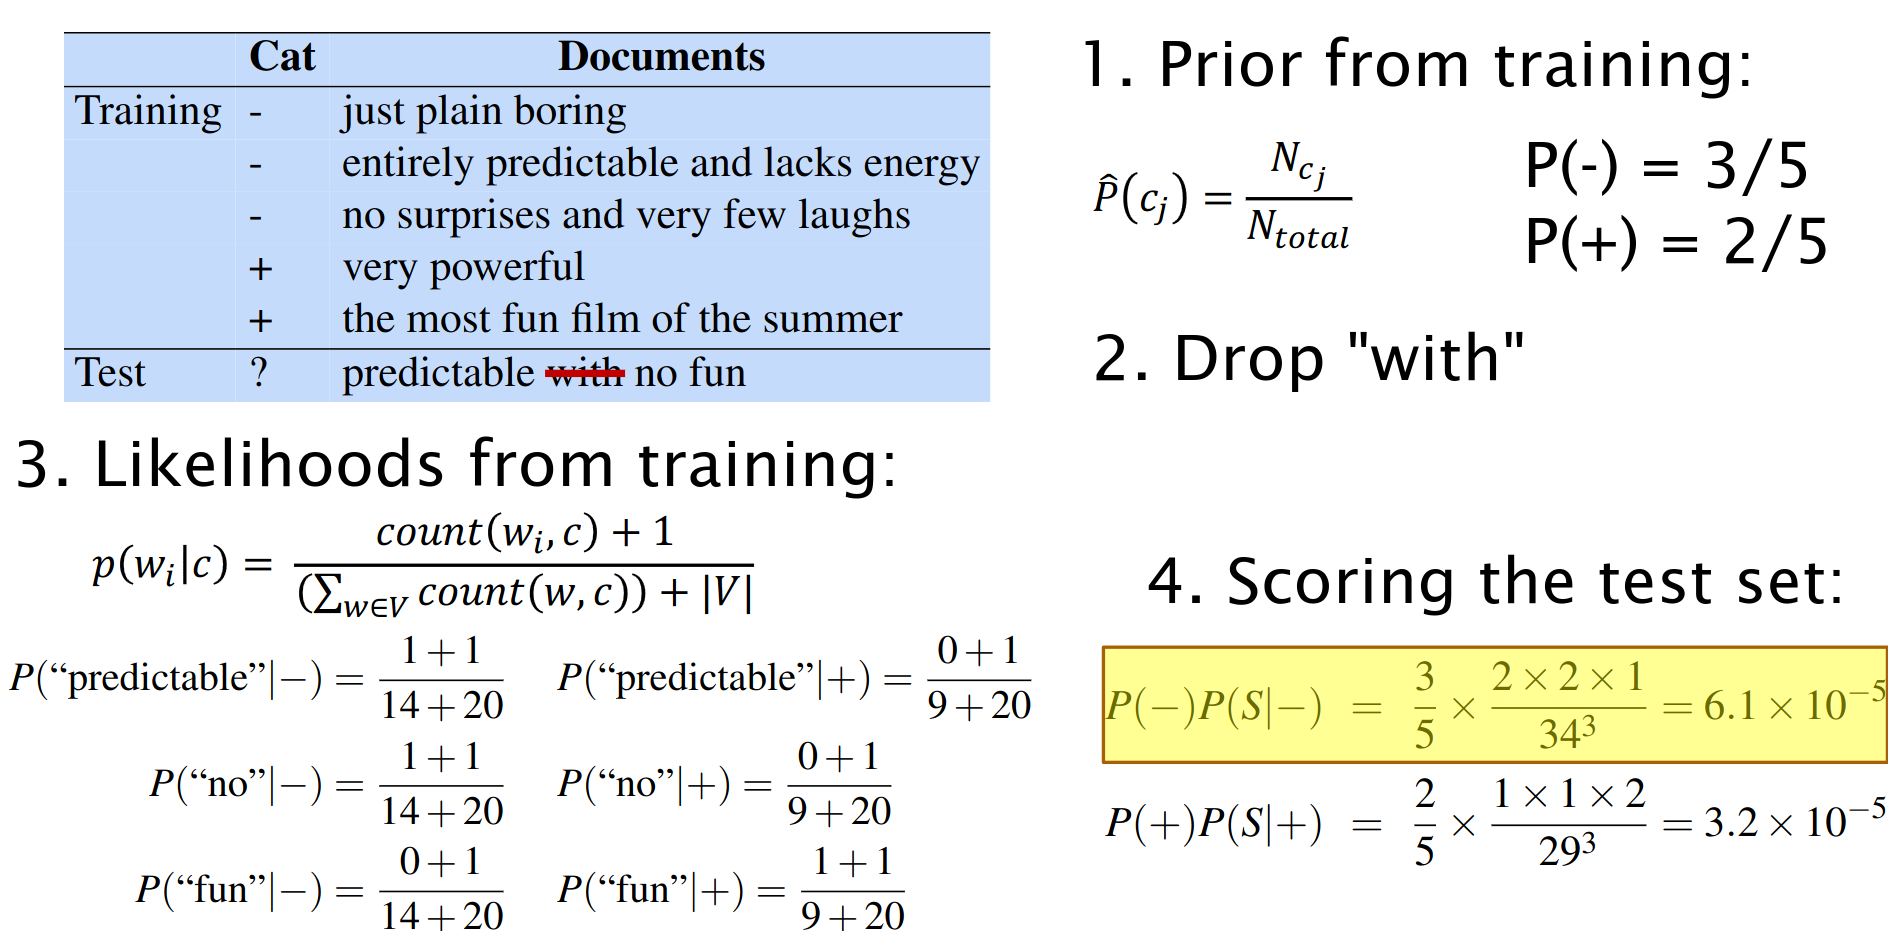
\includegraphics[scale = 0.23]{pics/naive_example.png}
\end{figure}

\end{frame}





\begin{frame}
\frametitle{Questions?}
%\vspace{1.5cm}
\begin{center}\LARGE Thanks for your Attention!\\ \end{center}



\end{frame}




\begin{frame}[allowframebreaks]\scriptsize
\frametitle{References}
\bibliography{bio}
\bibliographystyle{apalike}
%\bibliographystyle{flexbib}
\end{frame}  


%%%%%%%%%%%%%%%%%%%%%%%%%%%

\end{document}
